\documentclass[]{article}
\usepackage[a4paper, total={15cm,23cm}]{geometry}
\usepackage{fancyhdr}
\usepackage{graphicx}
\usepackage{amsmath}
\usepackage{amssymb}
\usepackage{xcolor}
\usepackage{tikz}
\usepackage{verbatim}
\usepackage{tcolorbox}
\usepackage{textcomp}
\usepackage{xcomment}
\usepackage{xstring}
\usepackage{array}
%opening
\title{PH 221 Week 1}
\author{Benjamin Bauml}
\date{Spring 2024}
\pagestyle{fancy}
\rhead{PH 221}
\chead{Spring 2024}
\lhead{Week 1}

% Version 2024-02-21
% Changes
% 2024-02-21 Added xstring package to enable smooth implementation of new \ModePage command.
% For Assignment, leave Purpose as 1. For Worksheet, set to 2. For Student Solution, set to 3. For Teacher Solution, set to 4.
\newcommand{\Purpose}{1}

\newcommand{\Exclusion}{0}
\newcommand{\PageTurn}{0}
\newcommand{\GrayProb}{0}
\newcommand{\Tipsy}{0}

% Assignment
\if\Purpose1
\renewcommand{\Exclusion}{1}
\fi
% Worksheet
\if\Purpose2
\renewcommand{\Exclusion}{1}
\renewcommand{\PageTurn}{1}
\fi
% Student Solution
\if\Purpose3
\renewcommand{\PageTurn}{1}
\renewcommand{\GrayProb}{1}
\fi
% Teaching Copy
\if\Purpose4
\renewcommand{\PageTurn}{1}
\renewcommand{\GrayProb}{1}
\renewcommand{\Tipsy}{1}
\fi

\if\Exclusion1
\xcomment{Title,Problem,ProblemSub,PassFig}
\fi

\def \NewQ {0}
\def \PForce {0}
\newcommand{\MaybePage}[1]{
	\def \PForce {#1}
	\if\PForce1
		\newpage
	\else
		\if\NewQ0
		\gdef \NewQ {\PageTurn}
		\else
		\newpage
		\fi
	\fi
}

\newcommand{\ModePage}[1]{
	\IfSubStr{#1}{\Purpose}{\newpage}{}
}

\newenvironment{Problem}[2][0]{%The first argument is optional, and if it is set to 1, the \newpage will be forced.
\MaybePage{#1}
\section*{#2}
\if\GrayProb1
\begin{tcolorbox}[colback=lightgray,colframe=lightgray,sharp corners,boxsep=1pt,left=0pt,right=0pt,top=0pt,bottom=0pt,after skip=2pt]
\else
\begin{tcolorbox}[colback=white,colframe=white,sharp corners,boxsep=1pt,left=0pt,right=0pt,top=0pt,bottom=0pt,after skip=2pt]
\fi
}{
\end{tcolorbox}\noindent
}

\newenvironment{ProblemSub}[1][0]{%The argument is optional, and if a string of numbers is entered into it, it will force a \newpage in any \Purpose that shows up in the string. For example, "13" would lead to the newpage being forced in modes 1 and 3.
\ModePage{#1}
\if\GrayProb1
\begin{tcolorbox}[colback=lightgray,colframe=lightgray,sharp corners,boxsep=1pt,left=0pt,right=0pt,top=0pt,bottom=0pt,after skip=2pt]
\else
\begin{tcolorbox}[colback=white,colframe=white,sharp corners,boxsep=1pt,left=0pt,right=0pt,top=0pt,bottom=0pt,after skip=2pt]
\fi
}{
\end{tcolorbox}\noindent
}

\newenvironment{PassFig}{\begin{figure}[h]}{\end{figure}}

\newcommand{\TeachingTips}[1]{
\if\Tipsy1
\begin{tcolorbox}[colback=lightgray,colframe=black]
#1
\end{tcolorbox}
\fi
}

\newenvironment{Title}{\maketitle}{}

\begin{document}
\begin{Title}
\begin{center}
	This material is borrowed/adapted from PH 201 Tutorial 1 for Fall 2020.
\end{center}
\end{Title}

\begin{Problem}{Activity 1}
	Add or subtract the following vectors.
\end{Problem}
In the solutions below, the first vector is colored {\color{blue}blue}, the second vector {\color{red}red}, and the resultant vector {\color{purple}purple}. Where applicable, both the ``tail-to-tip'' and the ``parallelogram'' method were used.

\begin{PassFig}
	\centering
	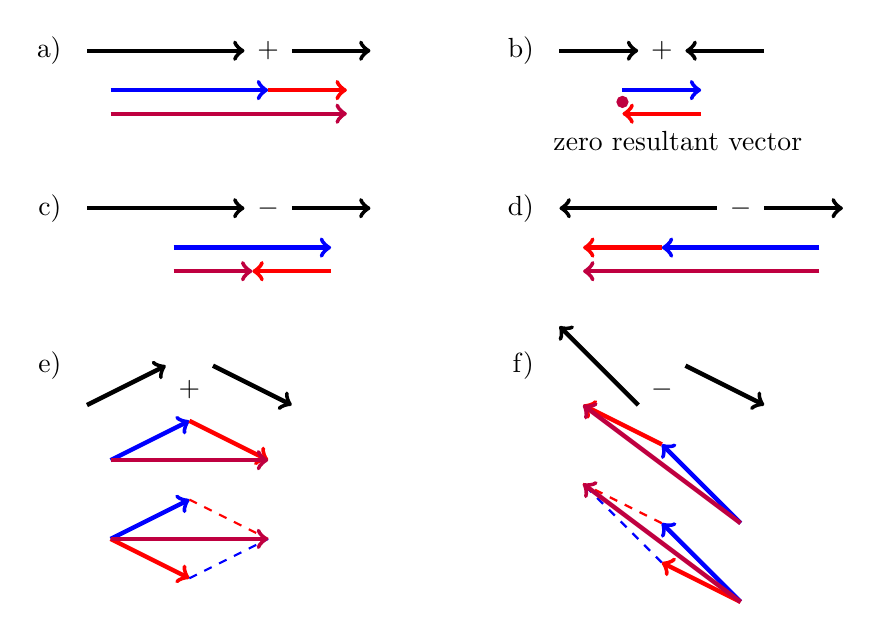
\begin{tikzpicture}
		\begin{scope}[shift={(0,0)}]
			\node[anchor=east] at (0,0) {a)};
			\draw[->,ultra thick,shift={(0.2,0)}] (0,0) -- (2,0);
			\node at (2.5,0) {$+$};
			\draw[->,ultra thick,shift={(2.8,0)}] (0,0) -- (1,0);
			\if\GrayProb1
			\draw[->,blue,ultra thick,shift={(0.5,-0.5)}] (0,0) -- (2,0);
			\draw[->,red,ultra thick,shift={(2.5,-0.5)}] (0,0) -- (1,0);
			\draw[->,purple,ultra thick,shift={(0.5,-0.8)}] (0,0) -- (3,0);
			\fi
		\end{scope}
		\begin{scope}[shift={(6,0)}]
			\node[anchor=east] at (0,0) {b)};
			\draw[->,ultra thick,shift={(0.2,0)}] (0,0) -- (1,0);
			\node at (1.5,0) {$+$};
			\draw[->,ultra thick,shift={(1.8,0)}] (1,0) -- (0,0);
			\if\GrayProb1
			\draw[->,blue,ultra thick,shift={(1,-0.5)}] (0,0) -- (1,0);
			\draw[->,red,ultra thick,shift={(1,-0.8)}] (1,0) -- (0,0);
			\filldraw[purple] (1,-0.65) circle (2pt);
			\node[anchor=north west] at (0,-0.9) {zero resultant vector};
			\fi
		\end{scope}
		\begin{scope}[shift={(0,-2)}]
			\node[anchor=east] at (0,0) {c)};
			\draw[->,ultra thick,shift={(0.2,0)}] (0,0) -- (2,0);
			\node at (2.5,0) {$-$};
			\draw[->,ultra thick,shift={(2.8,0)}] (0,0) -- (1,0);
			\if\GrayProb1
			\draw[->,blue,ultra thick,shift={(1.3,-0.5)}] (0,0) -- (2,0);
			\draw[->,red,ultra thick,shift={(2.3,-0.8)}] (1,0) -- (0,0);
			\draw[->,purple,ultra thick,shift={(1.3,-0.8)}] (0,0) -- (1,0);
			\fi
		\end{scope}
		\begin{scope}[shift={(6,-2)}]
			\node[anchor=east] at (0,0) {d)};
			\draw[->,ultra thick,shift={(0.2,0)}] (2,0) -- (0,0);
			\node at (2.5,0) {$-$};
			\draw[->,ultra thick,shift={(2.8,0)}] (0,0) -- (1,0);
			\if\GrayProb1
			\draw[->,blue,ultra thick,shift={(3.5,-0.5)}] (0,0) -- (-2,0);
			\draw[->,red,ultra thick,shift={(0.5,-0.5)}] (1,0) -- (0,0);
			\draw[->,purple,ultra thick,shift={(0.5,-0.8)}] (3,0) -- (0,0);
			\fi
		\end{scope}
		\begin{scope}[shift={(0,-4)}]
			\node[anchor=east] at (0,0) {e)};
			\draw[->,ultra thick,shift={(0.2,0)}] (0,-0.5) -- (1,0);
			\node at (1.5,-0.3) {$+$};
			\draw[->,ultra thick,shift={(1.8,0)}] (0,0) -- (1,-0.5);
			\if\GrayProb1
			\draw[->,blue,ultra thick,shift={(0.5,-0.7)}] (0,-0.5) -- (1,0);
			\draw[->,red,ultra thick,shift={(1.5,-0.7)}] (0,0) -- (1,-0.5);
			\draw[->,purple,ultra thick,shift={(0.5,-1.2)}] (0,0) -- (2,0);
			\draw[->,blue,ultra thick,shift={(0.5,-1.7)}] (0,-0.5) -- (1,0);
			\draw[->,red,ultra thick,shift={(0.5,-2.2)}] (0,0) -- (1,-0.5);
			\draw[dashed,red,thick,shift={(1.5,-1.7)}] (0,0) -- (1,-0.5);
			\draw[dashed,blue,thick,shift={(1.5,-2.2)}] (0,-0.5) -- (1,0);
			\draw[->,purple,ultra thick,shift={(0.5,-2.2)}] (0,0) -- (2,0);
			\fi
		\end{scope}
		\begin{scope}[shift={(6,-4)}]
			\node[anchor=east] at (0,0) {f)};
			\draw[->,ultra thick,shift={(0.2,0)}] (1,-0.5) -- (0,0.5);
			\node at (1.5,-0.3) {$-$};
			\draw[->,ultra thick,shift={(1.8,0)}] (0,0) -- (1,-0.5);
			\if\GrayProb1
			\draw[->,blue,ultra thick,shift={(1.5,-1.5)}] (1,-0.5) -- (0,0.5);
			\draw[->,red,ultra thick,shift={(1.5,-1)}] (0,0) -- (-1,0.5);
			\draw[->,purple,ultra thick,shift={(2.5,-2)}] (0,0) -- (-2,1.5);
			\draw[->,blue,ultra thick,shift={(1.5,-2.5)}] (1,-0.5) -- (0,0.5);
			\draw[dashed,blue,thick,shift={(0.5,-2)}] (1,-0.5) -- (0,0.5);
			\draw[dashed,red,thick,shift={(1.5,-2)}] (0,0) -- (-1,0.5);
			\draw[->,red,ultra thick,shift={(2.5,-3)}] (0,0) -- (-1,0.5);
			\draw[->,purple,ultra thick,shift={(2.5,-3)}] (0,0) -- (-2,1.5);
			\fi
		\end{scope}
	\end{tikzpicture}
\end{PassFig}

\begin{Problem}{Activity 2}
	A semi-truck travels 11 km in 7.5 minutes.
\end{Problem}
\begin{ProblemSub}
	a) What does the ratio (11 km)/(7.5 min) tell you about the truck's motion?
\end{ProblemSub}
This tells us the truck's average speed.
\begin{ProblemSub}
	b) What does the ratio (7.5 min)/(11 km) tell you about the truck's motion?
\end{ProblemSub}
This tells us how long it takes the truck to travel one kilometer.
\begin{ProblemSub}
	c) Find the truck's average speed in miles per hour, then in meters per second. Can you tell what type of road (school zone, residential area, freeway, German Autobahn, etc.) the truck should be traveling on?
\end{ProblemSub}
\[
\begin{split}
	\text{average speed (mph)} & = \frac{11\text{ km}}{7.5\text{ min}} = \frac{11\text{ km}}{7.5\text{ min}} \left(\frac{60 \text{ min}}{1\text{ h}}\right) = 88\text{ km/h} = 88\text{ km/h} \left(\frac{1\text{ mile}}{1.6 \text{ km}}\right) = 55\text{ mph} \\
	\text{average speed (m/s)} & = \frac{11\text{ km}}{7.5\text{ m}} = \frac{11\text{ km}}{7.5\text{ m}} \left(\frac{1000\text{ m}}{1\text{ km}}\right) \left(\frac{1\text{ min}}{60\text{ s}}\right) = 24.444 \text{ m/s} \approx 24\text{ m/s}
\end{split}
\]
55 mph is an appropriate freeway speed for a semi-truck.

Side Note: Notice that I truncated 24.444 to just 24. When figuring out how many decimal places to use, a decent rule of thumb (at this level) is to only include as many digits (not including leading zeros) as you are given in the least precise piece of data. Here, both 11 and 7.5 have two ``significant figures,'' so my final answer should only have two digits. If we had instead been given 11.0 and 7.50, we could assume enough reliability out to three digits to give our final answer as 24.4. However, if we had been given 11.0 and 7.5, we would still want to stick with two digits only, because 7.5 is less precise. Since every data point is assumed to be somewhat uncertain (limited by the accuracy of our measurements), we can't assume that 7.5 is precisely 7.50, nor that 7.50 is precisely 7.500.
\begin{ProblemSub}
	d) Find the time in seconds it takes the truck to travel one meter.
\end{ProblemSub}
\[
\text{time per meter} = \frac{7.5\text{ min}}{11\text{ km}} = \frac{7.5\text{ min}}{11\text{ km}} \left(\frac{1\text{ km}}{1000\text{ m}}\right) \left(\frac{60\text{ s}}{1\text{ min}}\right) = \frac{1}{24.444\text{ m/s}} \approx 0.041\text{ s/m}
\]
Side Note: 0.041 has two ``significant figures,'' since we do not count the leading zeros.

\begin{Problem}[1]{Activity 3}
	You are about to play a game of pool, so you and your opponent are lagging for the first shot. To lag, you must bounce the cue ball off of the far end of the table, and get it as close to the near end as possible without touching it. While preparing to strike, you accidentally give the cue ball a light tap, setting it in motion.
	
	Uh-oh! Through some bizarre accident, the pool table has become entirely frictionless! The cue ball slides toward the opposite end without rolling or slowing down.
	
	A spectator across the table from you decides that the midpoint is $ x=0 $ cm. Relative to her, the edge near you is at $ x = 127 $ cm, and the far edge is at $ x = -127 $ cm.
	
	It takes the cue ball 4 s to slide at constant velocity from $ x = 89 $ cm to $ x = 17 $ cm.
\end{Problem}
\begin{ProblemSub}
	a) What is its velocity?
\end{ProblemSub}
Since the ball is traveling at constant speed, we can find its velocity exactly by dividing the ball's displacement (from 89 cm to 17 cm) by the time it takes to undergo that displacement:
\[
v = \frac{\Delta x}{\Delta t} = \frac{x_{f}-x_{i}}{\Delta t} = \frac{17\text{ cm} - 89\text{ cm}}{4\text{ s}} = \frac{-72\text{ cm}}{4\text{ s}} = -18\text{ cm/s.}
\]
Note the sign; velocity is a vector, so it has magnitude (the speed, 18 cm/s) and direction (the negative sign, indicating that it is moving toward the negative side of the pool table, away from you). This is also seen in the displacement, which is negative.
\begin{ProblemSub}
	b) How long does it take the cue ball to slide from $ x = 17 $ cm to $ x = -127 $ cm?
\end{ProblemSub}
We can start with the same relationship between velocity, displacement, and elapsed time, and rearrange:
\[
v = \frac{\Delta x}{\Delta t} \implies \Delta t = \frac{\Delta x}{v} = \frac{x_{f}-x_{i}}{v} = \frac{-127\text{ cm}-17\text{ cm}}{-18\text{ cm/s}} = \frac{-144\text{ cm}}{-18\text{ cm}} = 8\text{ s.}
\]
\begin{ProblemSub}
	c) The cue rebounds from the far edge without losing speed. What is its position 10 s after it is at $ x = -127 $ cm?
\end{ProblemSub}
Note that $ v = +18\text{ cm/s} $ now. We once again take our expression for velocity and rearrange:
\[
\begin{split}
	v & = \frac{x_{f}-x_{i}}{\Delta t} \\
	x_{f}-x_{i} & = v\Delta t \\
	x_{f} & = x_{i} + v\Delta t = -127\text{ cm} + (18\text{ cm/s})(10\text{ s}) = 53\text{ cm.}
\end{split}
\]
Position is also a vector, so this positive number tells us that the ball is on the positive end of the table (on the near side of the midpoint, relative to you).


\begin{Problem}{Activity 4}
	Maria hikes 15.0 km at an angle of 30.0$ ^{\circ} $ north of east and then hikes 15.0 km southeast (an angle of 45.0$ ^{\circ} $ south of east). Let Maria's starting point be the origin of your coordinate system, the east-west axis be horizontal, and the north-south axis be vertical with east and north the positive directions.
\end{Problem}
\begin{ProblemSub}
	a) Draw a sketch, approximately to scale, showing the coordinate axes, Maria's two displacements, and her total displacement.
\end{ProblemSub}
\begin{figure}[h]
	\centering
	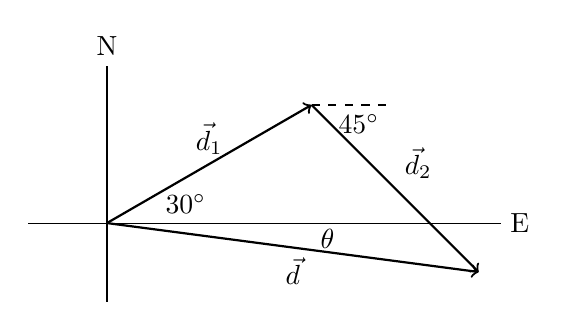
\begin{tikzpicture}
		\draw (0,-1) -- (0,2);
		\node[anchor=south] at (0,2) {N};
		\draw (-1,0) -- (5,0);
		\node[anchor=west] at (5,0) {E};
		\draw[->,thick] (0,0) -- ({3*cos(30)},{3*sin(30)});
		\node[anchor=south] at ({1.5*cos(30)},{1.5*sin(30)}) {$\vec{d}_{1}$};
		\node[anchor=south] at (1,0) {$30^{\circ}$};
		\draw[dashed] ({3*cos(30)},{3*sin(30)}) -- ({3*cos(30)+1},{3*sin(30)});
		\node[anchor=north] at ({3*cos(30)+0.6},{3*sin(30)}) {$45^{\circ}$};
		\draw[->,thick] ({3*cos(30)},{3*sin(30)}) -- ({3*cos(30)+3*cos(45)},{3*sin(30)-3*sin(45)});
		\node[anchor=south west] at ({3*cos(30)+1.5*cos(45)},{3*sin(30)-1.5*sin(45)}) {$\vec{d}_{2}$};
		\draw[->,thick] (0,0) -- ({3*cos(30)+3*cos(45)},{3*sin(30)-3*sin(45)});
		\node[anchor=north] at ({1.5*cos(30)+1.5*cos(45)},{1.5*sin(30)-1.5*sin(45)}) {$\vec{d}$};
		\node[anchor=north] at (2.8,0.05) {$\theta$};
	\end{tikzpicture}
\end{figure}

\noindent\textbf{Known:}
\begin{itemize}
	\item $ d_{1} = 15.0\text{ km};\ \theta_{1} = 30.0^{\circ} $
	\item $ d_{2} = 15.0\text{ km};\ \theta_{2} = -45.0^{\circ} $
\end{itemize}
\textbf{Find:} $ d,\ \theta $
\begin{ProblemSub}
	b) Find the east ($ x $) and north ($ y $) components of Maria's two displacements.
\end{ProblemSub}
\[
\begin{split}
	d_{1E} & = d_{1}\cos\theta_{1} = (15.0\text{ km})\cos30.0^{\circ} = 12.99\text{ km} \\
	d_{1N} & = d_{1}\sin\theta_{1} = (15.0\text{ km})\sin30.0^{\circ} = 7.50\text{ km} \\
	d_{2E} & = d_{2}\cos\theta_{2} = (15.0\text{ km})\cos(-45.0^{\circ}) = 10.61\text{ km} \\
	d_{2N} & = d_{2}\sin\theta_{2} = (15.0\text{ km})\sin(-45.0^{\circ}) = -10.61\text{ km} \\
\end{split}
\]
\begin{ProblemSub}
	c) Find the east ($ x $) and north ($ y $) components of Maria's total displacement.
\end{ProblemSub}
\[
\begin{split}
	d_{E} & = d_{1E} + d_{2E} = 12.99\text{ km} + 10.61\text{ km} = 23.60\text{ km} \\
	d_{N} & = d_{1N} + d_{2N} = 7.50\text{ km} + (-10.61\text{ km}) = -3.11\text{ km} \\
\end{split}
\]
\begin{ProblemSub}
	d) Find the magnitude and direction of Maria's total displacement.
\end{ProblemSub}
\[
\begin{split}
	d & = \sqrt{d_{E}^{2}+d_{N}^{2}} = \sqrt{(23.60\text{ km})^{2} + (-3.11\text{ km})^{2}} = 23.8\text{ km} \\
	\theta & = \tan^{-1}\left(\frac{d_{N}}{d_{E}}\right) = \tan^{-1}\left(\frac{-3.11\text{ km}}{23.60\text{ km}}\right) = -7.50^{\circ}
\end{split}
\]
\begin{ProblemSub}
	e) Check your answer to (d) against your sketch. Do they agree?
\end{ProblemSub}
Maria's displacement was 23.8 km at an angle of 7.50$ ^{\circ} $ south of east. This agrees with the sketch which shows a small angle below the x-axis. Note that the magnitude of her total displacement is only slightly greater than her total horizontal displacement because the angle is small.

In adding vectors by components, it is important to keep track of their signs. If we hadn’t had the negative sign in the north component of Maria’s second hike, our answer would have been much different (and wrong).

\begin{Problem}{Activity 5}
	Mary runs east at 6.0 km/h for 0.50 hr. She then turns around and runs west at 4.0 km/h for 1.0 h. Let east be the positive direction.
\end{Problem}
\begin{ProblemSub}
	a) Draw a motion diagram for Mary. Assume turning around takes negligible time.
\end{ProblemSub}
\begin{figure}[h]
	\centering
	
\begin{tikzpicture}[scale=1.5]
		\node[anchor=south] at (0,0) {\phantom{,}0\phantom{,}};
		\filldraw[black] (0,0) circle (2pt);
		\node[anchor=south] at (1,0) {1,6};
		\filldraw[black] (1,0) circle (2pt);
		\node[anchor=south] at (2,0) {\phantom{,}2\phantom{,}};
		\filldraw[black] (2,0) circle (2pt);
		\node[anchor=south] at (3,0) {\phantom{,}3\phantom{,}};
		\filldraw[black] (3,0) circle (2pt);
		\node[anchor=south] at (2.33,0) {\phantom{,}4\phantom{,}};
		\filldraw[black] (2.33,0) circle (2pt);
		\node[anchor=south] at (1.66,0) {\phantom{,}5\phantom{,}};
		\filldraw[black] (1.66,0) circle (2pt);
		%\node[anchor=south] at (1,0) {6};
		%\filldraw[black] (1,0) circle (2pt);
		\node[anchor=south] at (0.33,0) {\phantom{,}7\phantom{,}};
		\filldraw[black] (0.33,0) circle (2pt);
		\node[anchor=south] at (-0.33,0) {\phantom{,}8\phantom{,}};
		\filldraw[black] (-0.33,0) circle (2pt);
		\node[anchor=south] at (-1,0) {\phantom{,}9\phantom{,}};
		\filldraw[black] (-1,0) circle (2pt);
	\end{tikzpicture}
\end{figure}

Here, we have chosen $ \Delta t = 10 $ min. Other choices are also acceptable.
\begin{ProblemSub}
	b) How far does Mary run?
\end{ProblemSub}
To find how far she runs, we want the total distance she ran. Distance doesn't include directional information, so we just find how far she ran east and how far she ran west (two positive numbers) and add them together:
\[
\begin{split}
	d_{E} & = (6.0 \text{ km/h})(0.50\text{ h}) = 3.0\text{ km} \\
	d_{W} & = (4.0 \text{ km/h})(1.0\text{ h}) = 4.0\text{ km} \\
	d & = d_{E} + d_{W} = 3.0\text{ km} + 4.0\text{ km} = 7.0\text{ km.}
\end{split}
\]
\begin{ProblemSub}
	c) What is Mary’s displacement?
\end{ProblemSub}
Displacement is a vector, so we need to add the displacement of her eastward run (a positive number) to the displacement of her westward run (a negative number) to get the total displacement:
\[
\begin{split}
	\vec{d}_{E} & = (6.0 \text{ km/h})(0.50\text{ h}) = 3.0\text{ km} \\
	\vec{d}_{W} & = (-4.0 \text{ km/h})(1.0\text{ h}) = -4.0\text{ km} \\
	\vec{d} & = \vec{d}_{E} + \vec{d}_{W} = 3.0\text{ km} + (-4.0\text{ km}) = -1.0\text{ km}, \text{ i.e. } 1.0\text{ km, west.}
\end{split}
\]
\end{document}